\documentclass{article}
\usepackage[utf8]{inputenc}
\usepackage{graphicx}
\usepackage[paper=a4paper,left=3cm, right=3cm, top=2cm]{geometry}
\usepackage{blindtext}
\usepackage{multicol}
\usepackage{pgfplots}
\usepackage{float}
\usepackage{biblatex} %Imports biblatex package
\usepackage{amsmath}
\addbibresource{main.bib} %Import the bibliography file
\usepackage{array}

 
\pgfplotsset{compat = newest}

\title{\textbf{Inorganic scintillator based optic fiber dosimeter}}
\author{Neelkant Newra\\
\textit{Department of Biomedical Engineering} \\ National Institute of Technology, Raipur \\ Email: newra008@gmail.com\\}
\date{}

\begin{document}
\maketitle
\begin{abstract}\textbf{This study discuss the ongoing development in the field of inorganic scintillator based optic fiber dosimeters(IOSDFs) for medical radiotherapy dosimetry, mainly targeting real-time in vivo dosimetry. SFDs (scintillator-based optical fibre dosimeters) are small, electromagnetic interference-free, radiation-resistant, and durable. They've demonstrated a lot of promise for real-time in vivo radiotherapy dosimetry.Inorganic scintillators have a greater X-ray absorption and light output than organic scintillators. The stem effect may be easily removed with variable Inorganic scintillators  that have highest emission peaks in the red region of the spectrum. In this study we will look at various advantages and disadvantages of using inorganic scintillators for SFDs fabrication. We will be also discussing about various combination of IOSDFs used for different cases. } \\ \\
    \textbf{\textit{Keywords- Inorganic scintillators, dosimetry}} 
\end{abstract}

\begin{multicols}{2}

\section{Introduction}

Most modern medical diagnostic imaging methods that use x-rays or gamma rays use inorganic scintillators. The relatively high detection effectiveness of inorganic scintillators for harsh radiation explains this. However, the various diagnostic procedures differ significantly, and as a result, the radiation detector needs change as well. The scintillator specs do not always meet these requirements. One of the motivations for continuing scintillator Research and Development is to address this issue. The necessity for innovative, digital diagnostic systems with good image quality and a rapid picture acquisition time, as well as excellent quality real-time imaging systems for interventional radiology with minimal radiation dosage, are the other reasons. Traditional radiotherapy approaches have well-established safety and quality guidelines, however these protocols are being challenged by the aforementioned rapidly emerging radiotherapy technologies. Patients obtaining erroneous dosages while having radiation therapy using these novel radiotherapy procedures have been reported. This has raised worries about the time it takes for dosimetric equipment to catch up to treatment approaches. As a result, creating radiation dosimeters capable of real-time in vivo dose monitoring has gotten a lot of interest in the research community. Before looking at the development in the area of IOSFDs, lets use have some basic understanding of SFDs, there fundamentals, development, working , advantages and disadvantages.

\section{Fundamentals}
The fragment of scintillation material is coupled to an optical fibre in the standard SFDs arrangement. Figure 1 shows a simplified diagram of how SFDs operates in the presence of ionising radiation. When irradiated with a high-energy ionising beam, the scintillator undergoes a radioluminescence process (Fig. 1). An optical cable collects the light photons created in the scintillator and transmits them to the photon detector (e.g., photomultiplier, CCD camera, and spectrometer). A remote computer terminal can be used to analyse the output. Theoretically The emission of scintillation light is proportional to the dosage rate in theory. 

\begin{figure}[H]
    \centering
    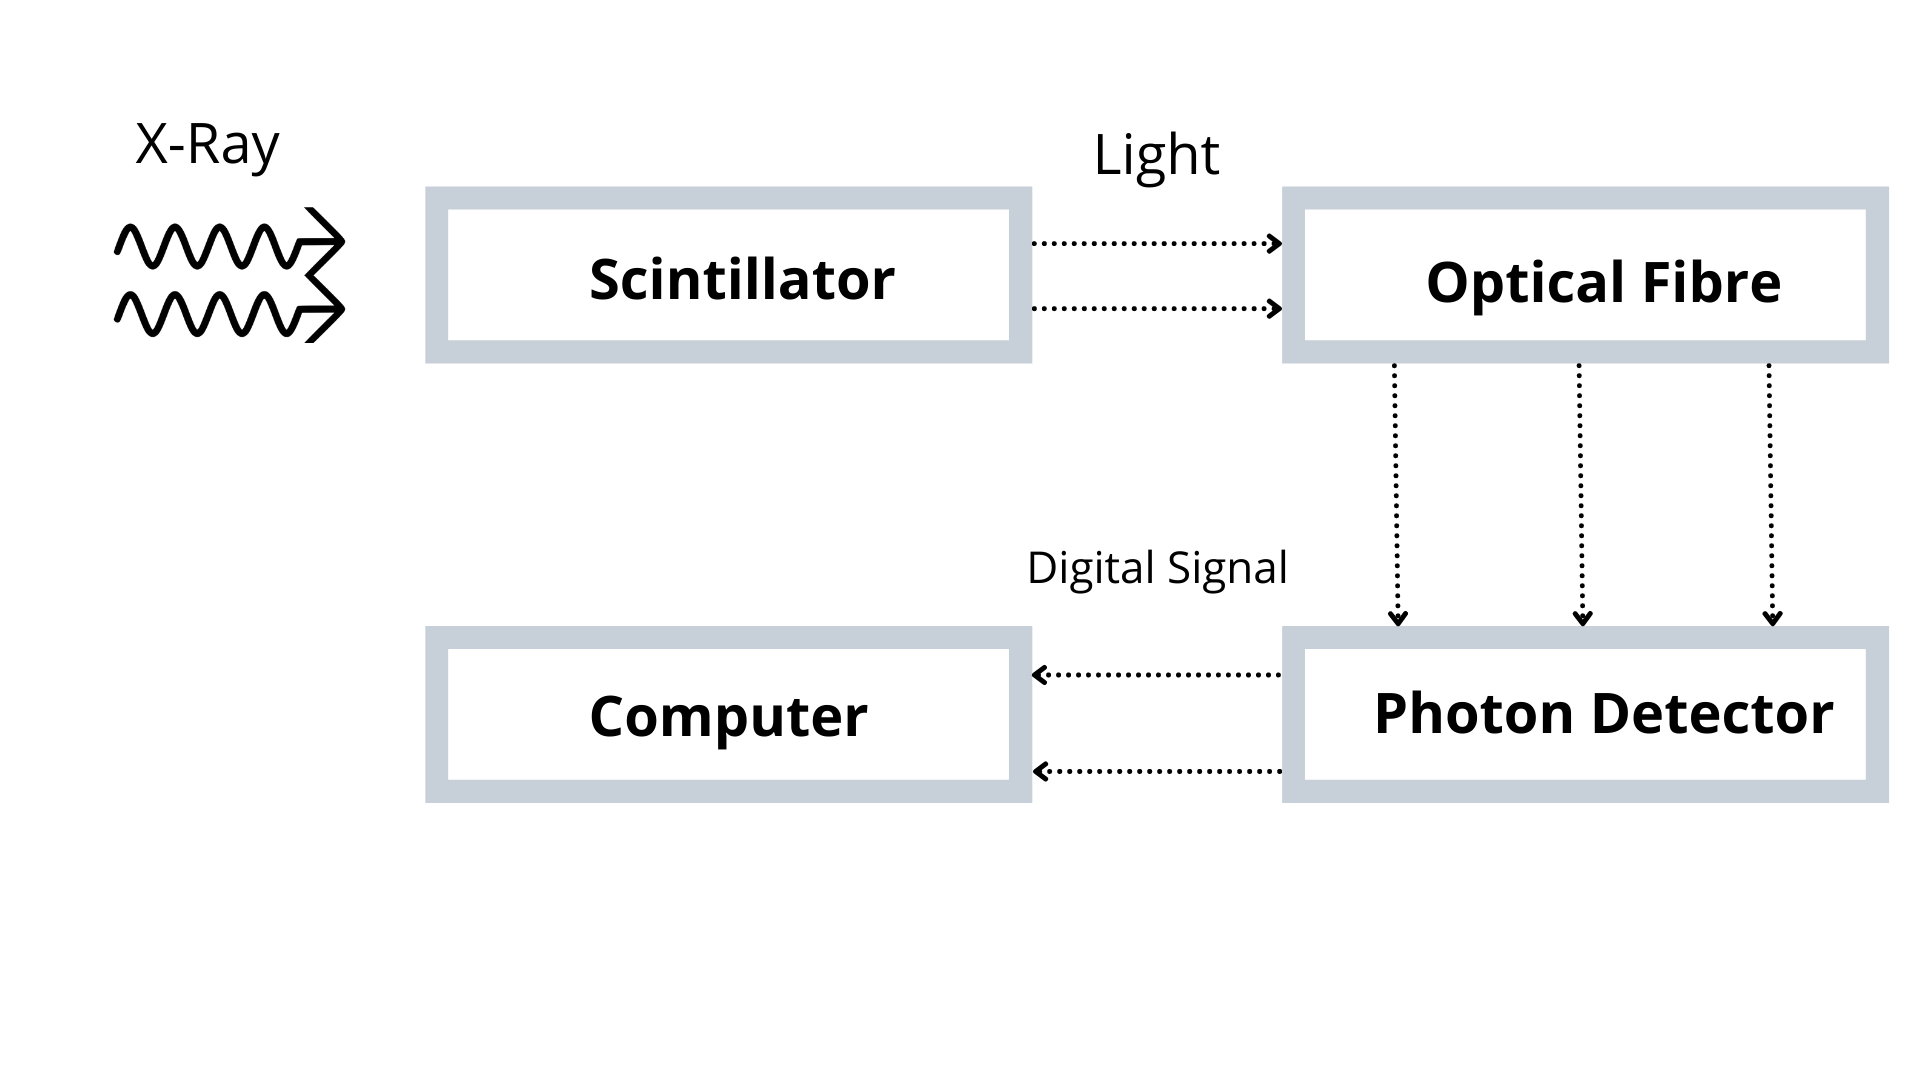
\includegraphics[width=6cm]{images/Fig1_Schematic.png}
    \caption{A simple schematic of the radiation detection process using SFDs}
    \label{fig:1}
\end{figure}

Overall, the scintillation light collecting efficiency and the scintillator's reaction to the incoming radiation particles determine the SFDs performance for oncology radiation measurement. The light collecting efficiency of scintillation is similar to the light extraction efficiency of LEDs(Light Emitting Diodes). It defines how well the optical fibre linked to the scintillator collects and transports scintillation light. The photons of scintilation light are emitted in all directions. To gather as many photons as feasible, an efficient coupling between the scintillation domain and the optical fibre with a small numerical aperture is required. Such linkage necessitated a sensitive setup of the IOSFD, which will be discussed and described later in the "Development of IOSFDs" section. We have touched the initial layer of how a SFDs works, lets look at the arrangement in a SFDs. 

\subsection{Development and Working of SFDs}
SFDs basically consist of Scintillator and PMT(Photo Multiplier Tube. Scintillator is a special kind of material medium in which if a charge particle enters it basically absorb the charge particle and leads to the creation of light, While Scintillation is the property of material medium, that when a external charge particle enter the medium, it absorb that energy and lead to the emission of light.

\end{multicols}





 
\end{document}
